\documentclass{beamer}
\usepackage{graphicx}
\usepackage[font=scriptsize]{caption}
\usepackage{mwe}
\usepackage[export]{adjustbox}
\usepackage[absolute, overlay]{textpos}
\usepackage{xcolor}
\usepackage{multimedia}
\usetheme{Madrid}  % You can change the theme by selecting a different one.

% Title slide information
\title{A Game Theory Simulation on the Battle of Gettysburg using Agent Based Modeling}
\author{Rubén Hernández O'kelly\\{\small rhernandezokelly@gmail.com}}
\institute{Institute for Computing in Research}
\date{\today}

\begin{document}


\setbeamertemplate{background}
{                  
  
\includegraphics[width=\paperwidth, height=\paperheight]{backgroundimage2.jpg}
}

% Title slide
\begin{frame}
  \titlepage
\end{frame}

% Slide with bullet points
\begin{frame}
  \frametitle{Peering into the Past: A Historical Context}
  \begin{itemize}
    \item American Civil War (1861-1865)
    \item Union vs. Confederate
    \item Strategic Importance: Why Gettysburg?
    \item Turning Point of the war
  \end{itemize}
  \begin{figure}
  \centering
      \includegraphics[width=6cm]{Battle_gettysburg_Image}
      \caption{The Battle of Gettysburg by Thure de Thulstrup}
      \label{fig:Battle}
  \centering
  \end{figure}    
\end{frame}

\begin{frame}
  \frametitle{Unraveling the puzzle: Simulation Objectives}
  \begin{itemize}
    \item{Simulate the battle using Game Theory and Agent Based Modeling}
    \item{Strategic decision-making of agents using Game Theory}
    \item{Validating the simulation}
  \end{itemize}
  \begin{figure}
    \centering
      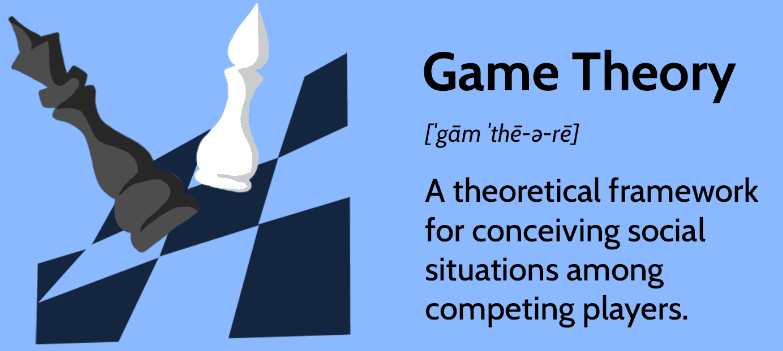
\includegraphics[width=6cm]{GameTheoryImage}
      \caption{Investopedia}
      \label{fig:Game_Theory}
    \centering
  \end{figure}
\end{frame}  

\begin{frame}
  \frametitle{The Game is on}
  \begin{itemize}
    \item{Game theory and ABM}
    \item{Implementation}
    \item{Merge}
  \end{itemize}  

\end{frame}

\begin{frame}
  \frametitle{Model and Agents}
  \begin{itemize}
    \item{Matplotlib}
    \item{Agents}
    \item{Blue: Union}
    \item{Red: Confederation}
  \end{itemize}
%image of battlefield

\end{frame}

\begin{frame}
  \frametitle{Simulation Process}
  \begin{itemize}
  \item{Simulation}
  \end{itemize}
  \movie{\includegraphics[width=\textwidth]{Battle_gettysburg_Image}}{SimVid.webm}
\end{frame}

\begin{frame}
  \frametitle{Results and Analysis}
  \begin{itemize}
  \item{Results}
  \end{itemize}
  \begin{figure}
    \centering
    
\includegraphics[width=6cm]{Battle_1.png}
    \caption{Results}
    \label{fig:Simulation}
    \centering
  \end{figure}

  
\end{frame}

\begin{frame}
  \frametitle{Summary and Future works}
  \begin{itemize}
  \item{Summary}
  \item{Future Works}
  \end{item}
\end{frame}

\begin{frame}
  \frametitle{References}
  \bibliographystyle{elsarticle-harv} 
  \begin{thebibliography}{9}
  \bibitem  Gettysburg Historic Crossroads (July 15th, 2023) \emph {https://www.gettysburgpa.gov/history/slideshows/battle-history}, Pennsylvania Gov.
  \bibitem  Gettysburg (July 15th, 2023) \emph {https://www.gettysburgpa.gov/history/slideshows/battle-history}, American Battlefield Trust.
  \bibitem  NashPy Documentation (July 11th, 2023) \emph{https://nashpy.readthedocs.io/en/stable/tutorial/index.html}
  \end{thebibliography}
\end{frame}
\end{document}
